\chapter{Related Work}\label{sec:related-work}
This thesis brings together two different domains, and in both domains research has been published on sequence prediction. First in the context of processes and second in the context of natural language.
\marginpar{Furthermore they may be some research on Neural Network Architecture?!}

%\section{Process prediction}
Hauder et al. mention numerous research challenges in the domain of ACM, among them an active support system for knowledge workers \cite{hauder2014}.
The need for such a system is emphasized by Francescomarino et al. in their literature review, where it has been found that few prediction approaches target the next activity \cite{francescomarino2018}.\\

\marginpar{CoCaMa is an abbreviation for a project called Collaborative Case Management, which appears to be retired: \href{http://archive.li/uZFnN}{archive.li/uZFnN}}
An example for how such a system might look like is given by Huber, who has developed a next-step recommendation system serving different case goals.
The system is prototypically implemented as CoCaMa, a prototypical case management application. The system has been evaluated with 25 hand-made case logs.\\

Building upon each other are the works by Evermann et al. \cite{evermann2016} and Schönig et al. \cite{schoenig2018}. Evermann et al. have successfully demonstrated the good performance of long-short-term memory (LSTM) neural networks in predicting the next activity on BPI datasets from 2012 and 2013. Their approach did not take into account specific case data attributes however. How making use of this contextual information can improve the prediction accuracy even more, has been shown by Schönig et al. \cite{schoenig2018} on BPI datasets from 2017. Furthermore, Schönig et al. have explored data preparation methods for supporting the model during learning.
This thesis can thus be seen as the continuation of these two works.

Similar to Schönig et al., Polato et al. make use of environmental information in their work for improving the prediction of the remaining time of business process instances \cite{polato2014}.\\

Metzger et al. predict run-time of a case by comparing and combining different prediction models into a model ensemble. Then, the members of the ensemble are selected based on their predictive performance measures. This allows taking into account costs of false predictions \cite{metzger2015}.\\

Francescomarino et al. have performed clustering in the preprocessing phase of model training and prediction. Having clustered the training data, one model was created and trained for each cluster. For obtaining a prediction, the cluster for a new data item is found from which the corresponding model is selected.
This approach was evaluated on the accuracy of predicate fulfillment with two different clustering methods (k-means and DBSCAN) and two different prediction models (decision trees and random forests) \cite{francescomarino2015}.
A further evaluation criteria was \textit{earliness}, i.e. at which point in time the correct result could be determined.

Continuing Francescomarinos approach and training a neural network for every cluster was considered at the beginning of this thesis but foregone because of possibility to use embedding layers.\\

Colocated with the International Conference in Grammatical Inference 2016 (ICGI) was a competition called SPiCE\ "about guessing the next element in a sequence" \cite{web:spice}.
Most entries submitted to the competition used RNNs with LSTM cells to predict the next word of a sentence.
The winning submission by Shibata et al. used a bipartite network architecture training separate layers on different features of the same row. The results of separate input layers are merged in the middle hidden layers to produce a single output \cite{shibata2016bipartite}. This architecture is depicted in \autoref{fig:spice-winner-architecture}.
While one half of the layers was trained on the most recent word of the sentence, the other half was trained on the prefix of that word. As this prefix could have been on any length, Shibata et al. propose a binary bag-of-words encoding. This encodes the states of a SP-2 automaton.

\begin{figure}
    \centering
    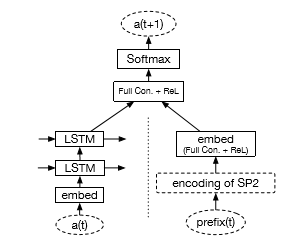
\includegraphics[height=.5\textwidth]{gfx/spice-winner-architecture.png}
    \caption{The neural network architecture of the winning submission at the SPiCE competition \cite{shibata2016bipartite}.}
    \label{fig:spice-winner-architecture}
\end{figure}

SP-$k$ languages are used to describe certain long-term dependencies through forbidding subsequences. If $\langle a,b \rangle$ is forbidden, then no $b$ may ever occur after $a$. A deterministic finite automaton (DFA) can also be used to characterize SP-$k$ languages, if its states encode the subsequences of size $k-1$  present in the previous prefixes \cite{heinz2010estimatingSP}. \autoref{tab:sp2-encoding} illustrates this encoding with a small example.

\begin{table}
    \centering
    \begin{tabular}{cclccccc}
        \hline
          &      &              & \multicolumn{5}{c}{SP-2 vector}\\
        t & a(t) & prefix(a(t)) & [a & b & c & d & e]\\
        \hline
        0 & a    & a            & [1 & 0 & 0 & 0 & 0]\\
        1 & d    & ad           & [1 & 0 & 0 & 1 & 0]\\
        2 & a    & ada          & [1 & 0 & 0 & 1 & 0]\\
        3 & c    & adac         & [1 & 0 & 1 & 1 & 0]\\
        4 & d    & adacd        & [1 & 0 & 1 & 1 & 0]\\
        \hline
    \end{tabular}
    \caption{Exemplary SP-2 encoded prefixes with $\sum=\{a,b,c,d,e\}$, abridged from Shibata et al.  \cite{shibata2016bipartite}. \textbf{TODO USE SEQUENCE NOTATION HERE}}
    \label{tab:sp2-encoding}
\end{table}